\begin{figure}[tb]
  \centering
  \begin{subfigure}{0.155\linewidth}
  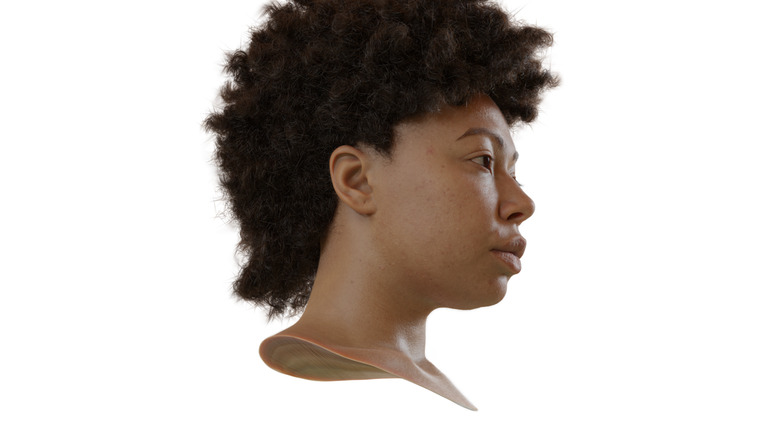
\includegraphics[width=\linewidth]{images/renders/khady_rgb_31.jpg}
  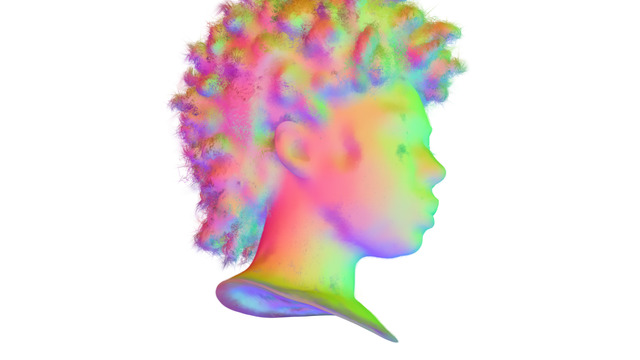
\includegraphics[width=\linewidth]{images/normals/khady_normals_31.jpg}
  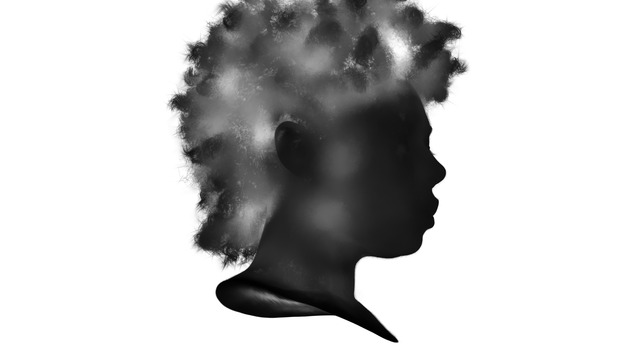
\includegraphics[width=\linewidth]{images/frosting_size/khady_size_31.jpg}
  \end{subfigure}
  %
  \hfill
  %
  \begin{subfigure}{0.155\linewidth}
  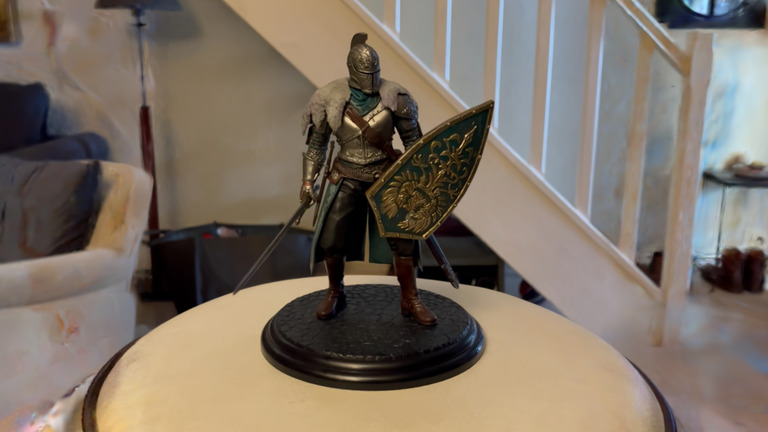
\includegraphics[width=\linewidth]{images/renders/faraam0_rgb_14.jpg}
  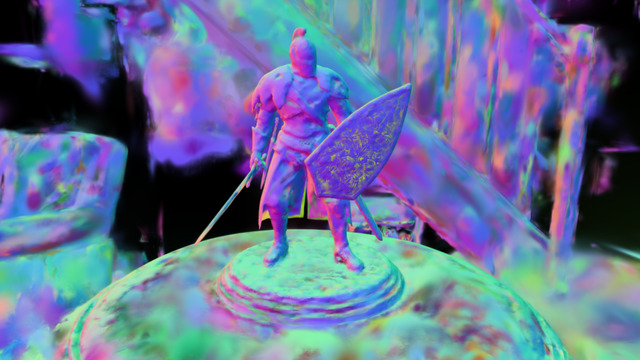
\includegraphics[width=\linewidth]{images/normals/faraam0_normals_14.jpg}
  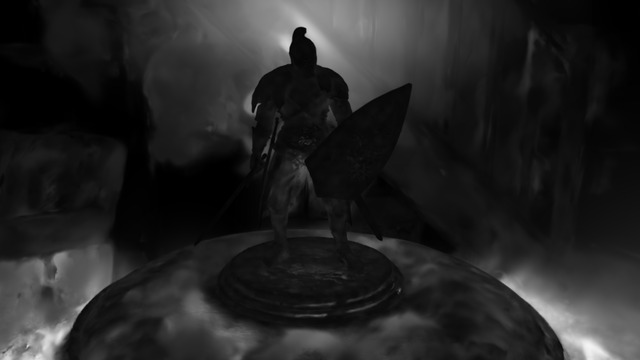
\includegraphics[width=\linewidth]{images/frosting_size/faraam0_size_14.jpg}
  \end{subfigure}
  %
  \hfill
  %
  \begin{subfigure}{0.155\linewidth}
  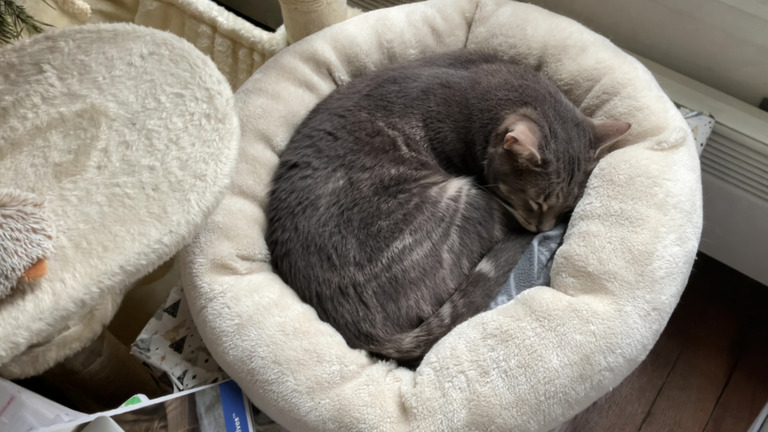
\includegraphics[width=\linewidth]{images/renders/sirius1_rgb_52bis.jpg}
  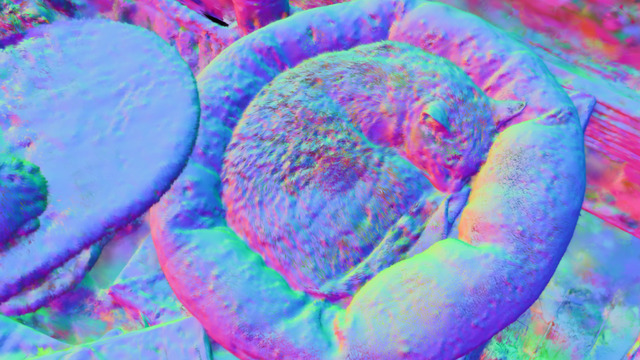
\includegraphics[width=\linewidth]{images/normals/sirius1_normals_52_bis.jpg}
  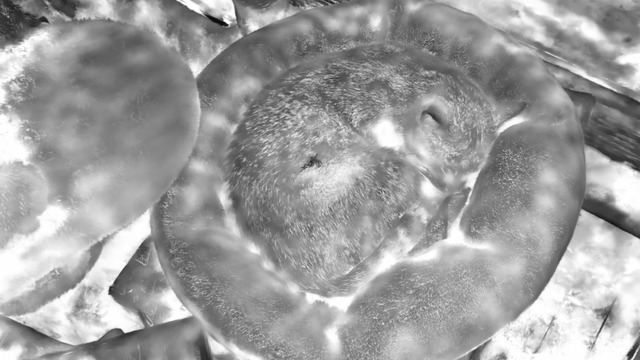
\includegraphics[width=\linewidth]{images/frosting_size/sirius1_size_52_ter.jpg}
  \end{subfigure}
  %
  \hfill
  %
  \begin{subfigure}{0.155\linewidth}
  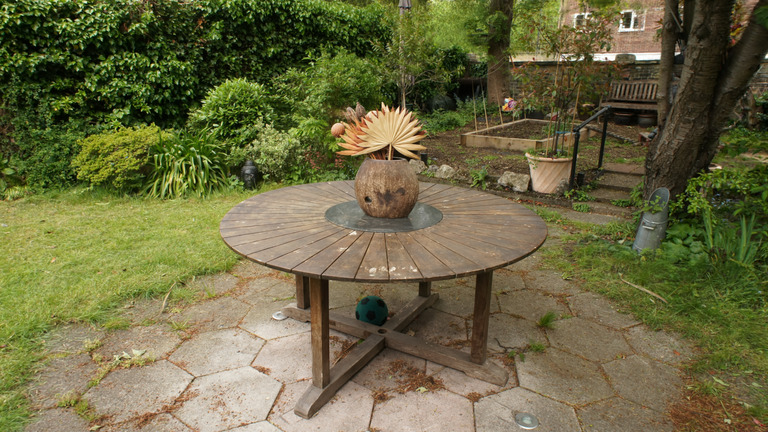
\includegraphics[width=\linewidth]{images/renders/garden_rgb_31.jpg}
  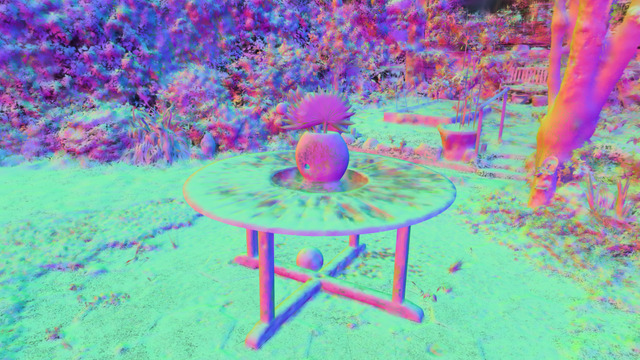
\includegraphics[width=\linewidth]{images/normals/garden_normals_31bis.jpg}
  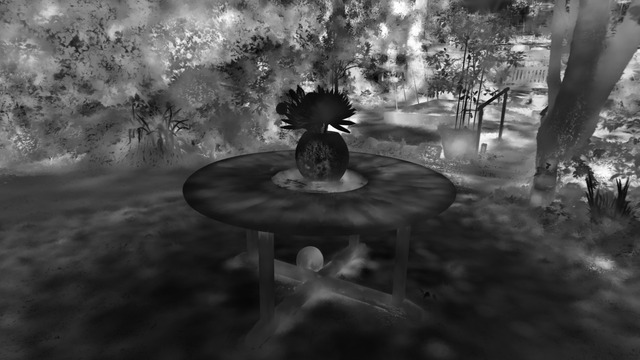
\includegraphics[width=\linewidth]{images/frosting_size/garden_size_31bis.jpg}
  \end{subfigure}
  %
  \hfill
  %
  \begin{subfigure}{0.155\linewidth}
  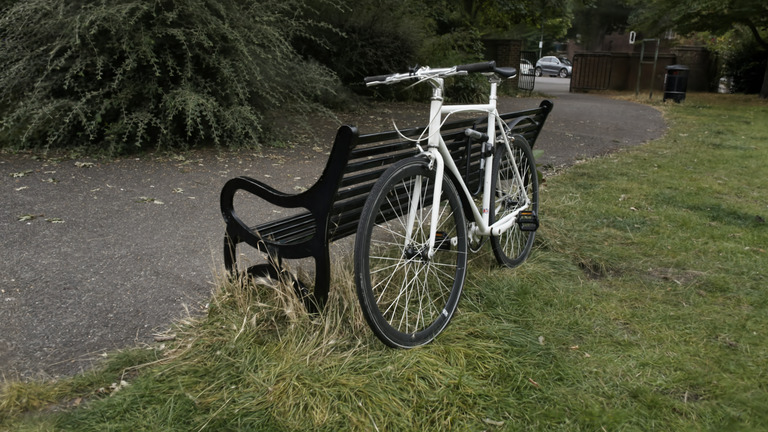
\includegraphics[width=\linewidth]{images/renders/bicycle_rgb_52.jpg}
  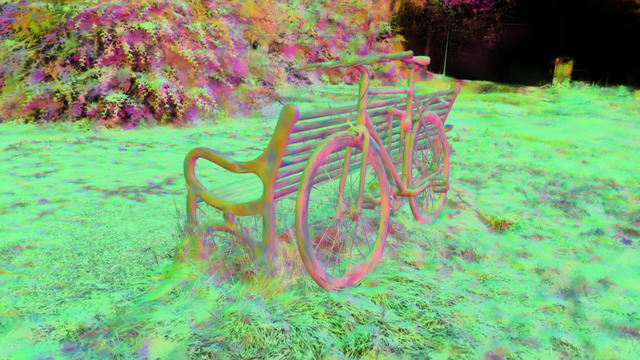
\includegraphics[width=\linewidth]{images/normals/bicycle_normals_52bis.jpg}
  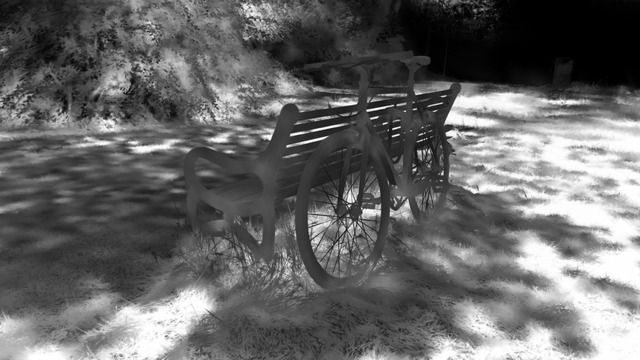
\includegraphics[width=\linewidth]{images/frosting_size/bicycle_size_52bis.jpg}
  \end{subfigure}
  %
  \caption{
  \textbf{Rendering complex scenes with Frosting.} First row: Renderings, Second row: recovered normal maps, Third row: estimated Frosting thickness. Note that the Frosting is thick on fuzzy materials such as the hair and the grass, as expected, and very thin on flat surfaces such as the table on the fourth column.
  }
  \label{fig:frosting-renders}
\end{figure}